\documentclass{article}

\usepackage{lmodern}
\usepackage{hyperref}
\usepackage{amsmath}
\usepackage{amssymb}
\usepackage[T1]{fontenc}
\usepackage{fancyhdr}
\usepackage{color,graphicx}
\pagestyle{fancy}
\lhead{Anirudhan J. Rajagopalan --- ajr619}

\begin{document}

\title{Kernel Based Approaches for Change-Point Detection --- Report 1 \\ Spectral density \& Peridogram}
\date{March 1, 2016}
\author{Anirudhan J. Rajagopalan, ajr619}

\maketitle

\newpage

\section{Spectral density}
\subsection{Linear combination of sinusoidals}
Suppose we have a time series defined as 
\begin{align}
  X_{t} = \sum_{j = 1}^{k} (A_{j} \cos(\omega_{j}t) + B_{j} \sin(\omega_{j}t)), \qquad 0 < \omega_{1} < \cdots < \omega_{k} < \pi
\end{align}

The time series is given in Figure~\ref{fig:sd2_ts} The timeseries is generated with values 
\begin{align*}
  K =& 2\\ 
  \omega =& [ 1.57079633, 0.78539816],\\
  A =& [-0.31201389 -1.04898091] \text{\quad and} \\
  B =& [-0.33909457 -0.1755208 ].
\end{align*}

\begin{figure}[ht!]
  \centering
  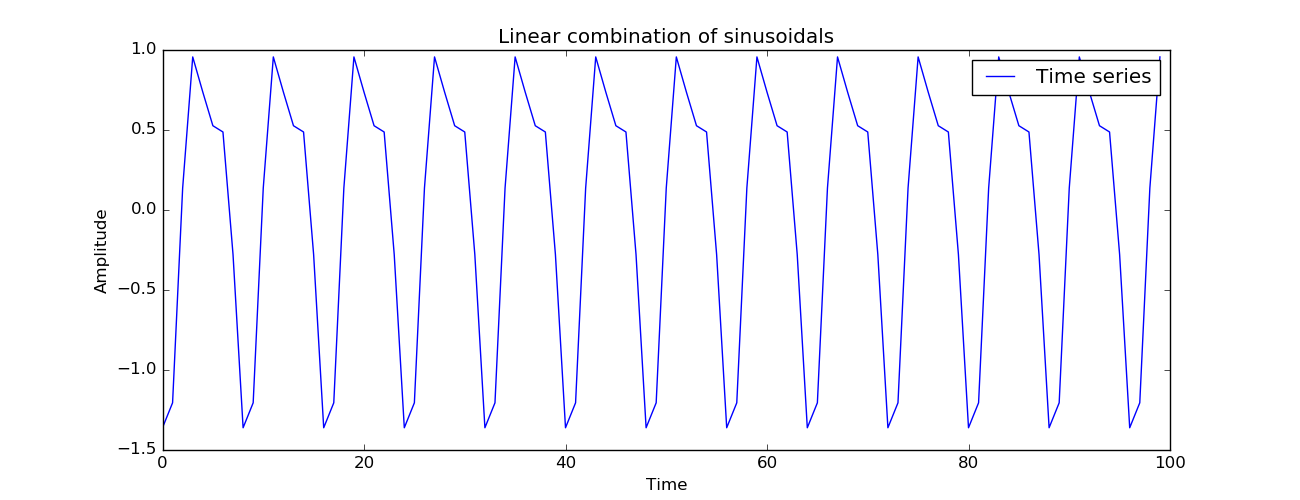
\includegraphics[width=1\textwidth]{images/spectral_density_2/ts}
  \caption{Timeseries generated by Linear combination of sinusoidals.~\label{fig:sd2_ts}}
\end{figure}

The Auto Covariance Function (ACVF) of this time series is given by
\begin{align}
  \gamma(h) = \sum_{j=1}^{k} \sigma^{2}\cos(\omega_{j}h)
\end{align}

as defined in~\cite{itsf}. 

The ACVF as a function of $h$ is shown in Figure~\ref{fig:sd2_acvf}

\begin{figure}[ht!]
  \centering
  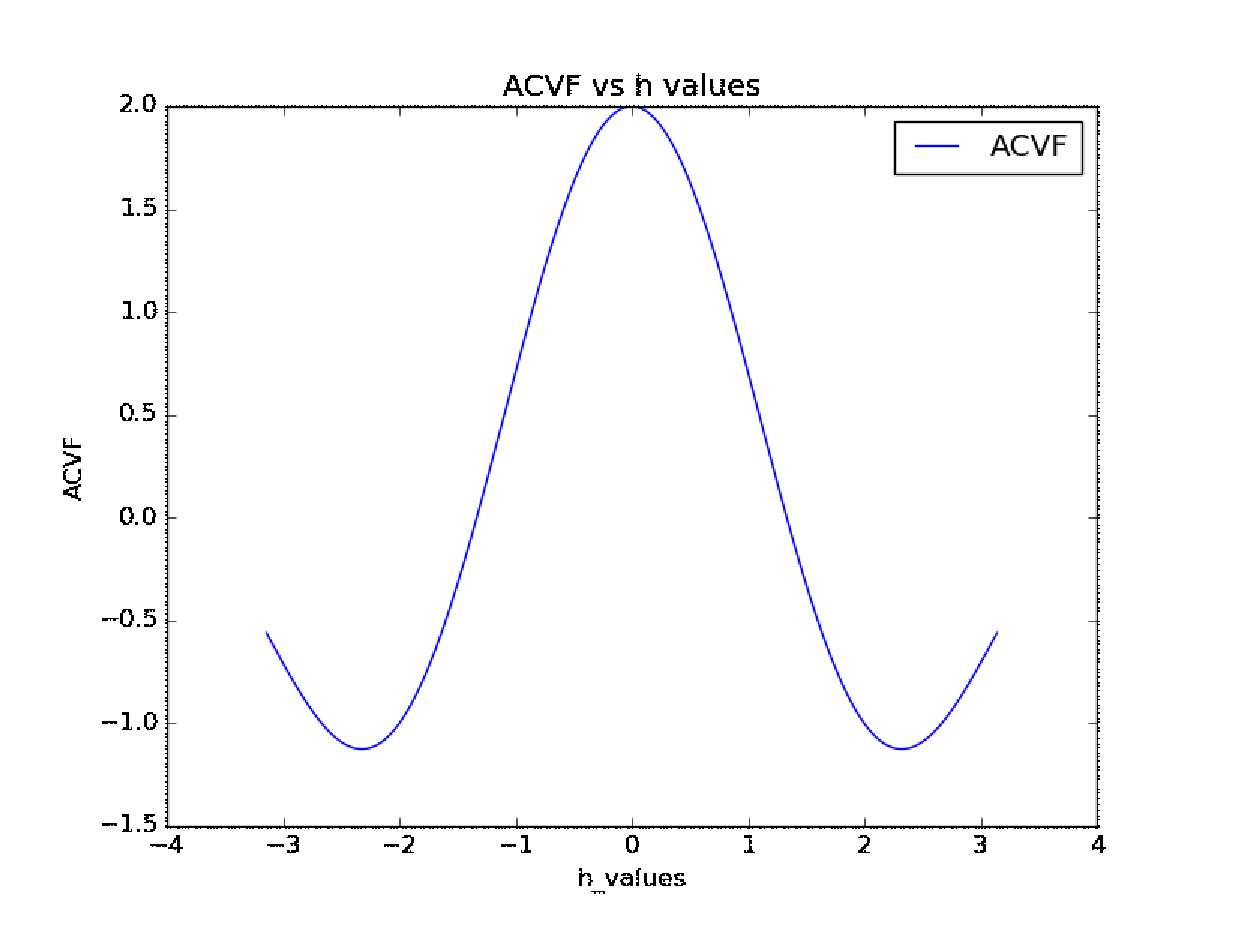
\includegraphics[width=0.75\textwidth]{images/spectral_density_2/acvf}
  \caption{ACVF for the timeseries defined in Figure~\ref{fig:sd2_ts}.\label{fig:sd2_acvf}}
\end{figure}

Also the spectral density is given by:

\begin{align}
  F_{j}(\lambda) = \begin{cases}
    0.0 & \text{if \qquad } \lambda < -\omega_{j},\\
    0.5 & \text{if \qquad } -\omega_{j} \le \lambda < \omega_{j},\\
    1.0 & \text{if \qquad } \lambda \ge \omega_{j}.
  \end{cases}
\end{align}

The spectral density of the function for $h \in (-\pi, \pi)$ is shown in Figure~\ref{fig:sd2_sd}.

\begin{figure}[ht!]
  \centering
  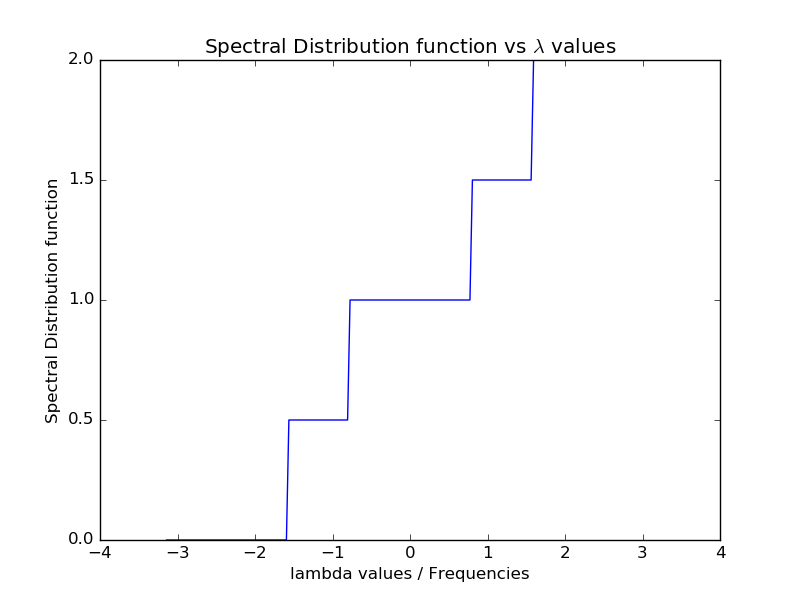
\includegraphics[width=0.75\textwidth]{images/spectral_density_2/sd}
  \caption{Spectral density for the timeseries defined in Figure~\ref{fig:sd2_ts}.\label{fig:sd2_sd}}
\end{figure}

\subsection{Observation and Questions}
\begin{enumerate}
  \item An important observation is that we didn't use the samples to find ACVF since we know $\omega$, and $\lambda$.
  \item The value of sigma which is not used for generating the time series is used for calculating ACVF\@.
\end{enumerate}

\section{Peridogram}
We can find the peridogram of a time series given by samples ${x_{1}, \ldots, x_{n}}$ by
\begin{align}
  I_{n}(\lambda) = \frac{1}{n} \lvert\sum_{t=1}^{n} x_{t}e^{-it\lambda} \rvert^{2}
\end{align}

The peridogram of the time series defined given in Figure~\ref{fig:sd2_ts} is given in Figure~\ref{fig:sd2_peri1}

\begin{figure}[ht!]
  \centering
  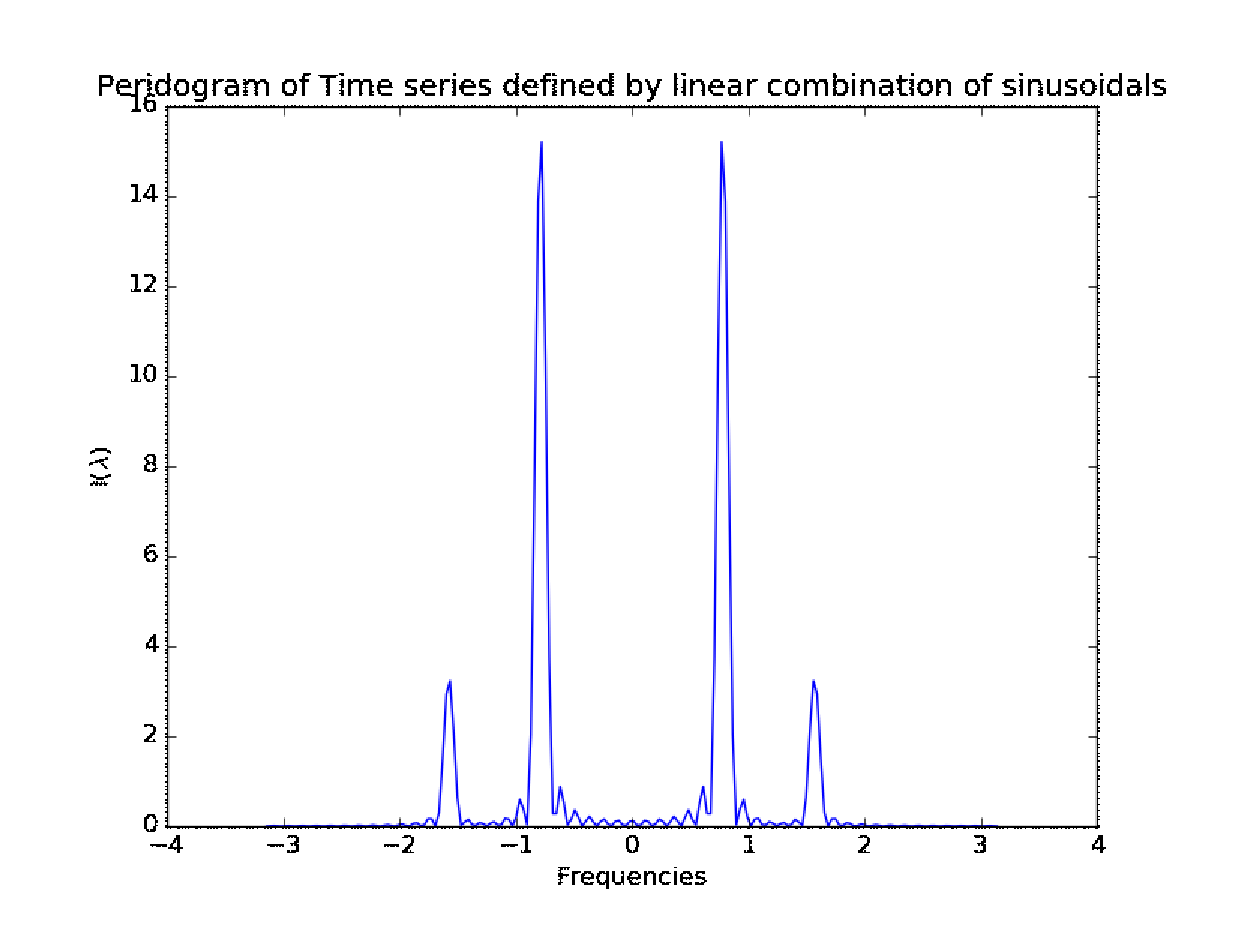
\includegraphics[width=0.75\textwidth]{images/spectral_density_2/peri1}
  \caption{Peridogram for the timeseries defined in Figure~\ref{fig:sd2_ts}.\label{fig:sd2_peri1}}
\end{figure}

As can be clearly seen from Figure~\ref{fig:sd2_peri1}, the peridogram has high values of $I$ which corresponds to the frequencies that make up the signal.

We also ran several other experiments using time series generated by stacking multiple sinusoidal signals with varying frequencies.  Below is a time series which is a combination of sinusoidals with frequencies$(1, 2, 3)$ stacked one after the other along with gaussian noise.

\begin{figure}[ht!]
  \centering
  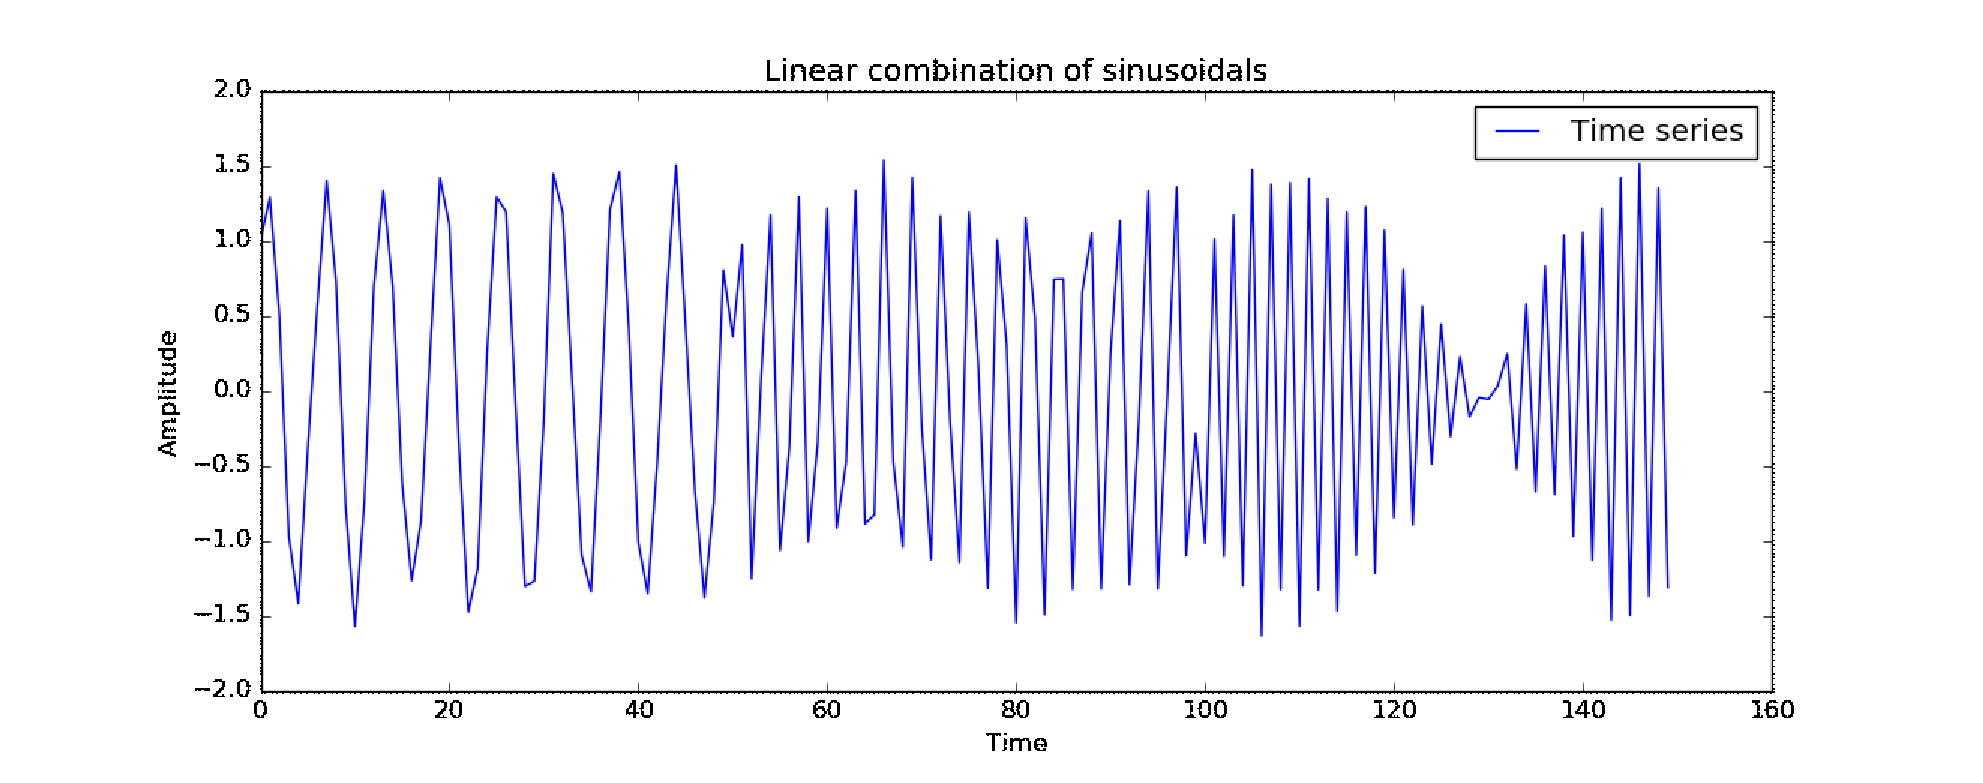
\includegraphics[width=1\textwidth]{images/spectral_density_2/ts2}
  \caption{Time series formed by concatenating 50 samples generated by linear combination of sinusoidals of frequencies 1, 2, and 3.  The change points are at time t = 50, and 100.\label{fig:sd2_ts2}}
\end{figure}

The peridogram for this time series is calculated for values of lambda ranging from $(-\pi, \pi)$.

\begin{figure}[ht!]
  \centering
  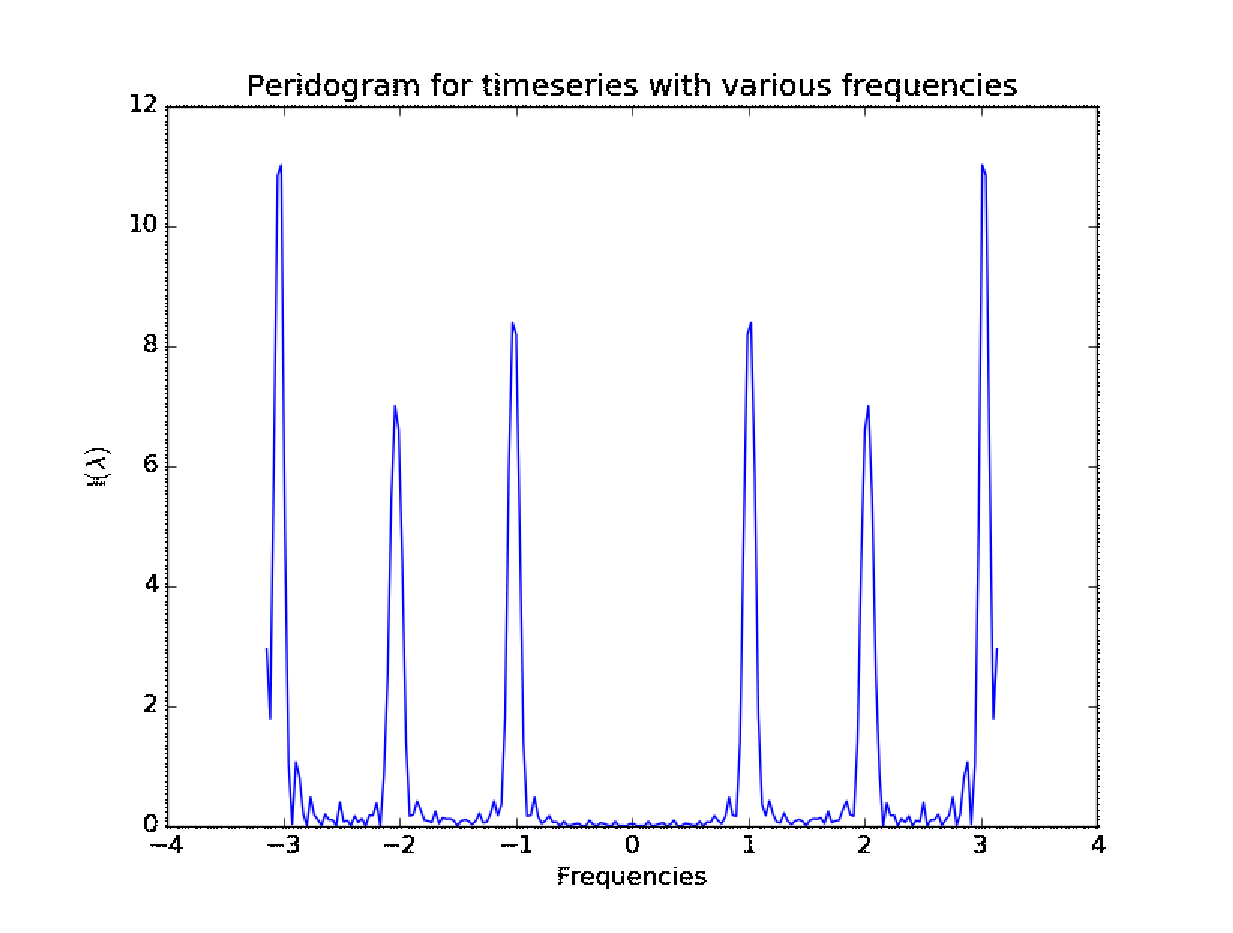
\includegraphics[width=0.75\textwidth]{images/spectral_density_2/peri2}
  \caption{Peridogram for time series shown in Figure~\ref{fig:sd_ts2}.\label{fig:sd2_peri2}}
\end{figure}

We also foudn the peridogram by using a sliding window of width 25 over the time series.

\bibliographystyle{plain}
\bibliography{references}
\end{document}
